%%%%%%%%%%%%%%%%%%%%%%%%%%%%%%%%%%%%%%%%%
% Trace Analysis and Monitoring
% 
% $Date$
% $Rev$:
% $Author$

\chapter{\KiekerTraceAnalysis{}: Monitoring, Analyzing \& Visualizing Traces}\label{chap:aspectJ}

This chapter will show in Section~\ref{sec:aspectJ:annotation} how
to use AspectJ to mark methods to be monitored with a simple annotation
in order to avoid the manual monitoring as seen in Chapter~\ref{chap:example}
and \ref{chap:componentsMonitoring}. Once the methods are marked, the AspectJ-Weaver-Agent
will surround the calls with the necessary code during runtime, similar
to the manually inserted instrumentation code used in Section~\ref{sec:example:monitoring}.
An alternative solution will be shown as well in Section~\ref{sec:aspectJ:fullweaving}, %
where the methods to be instrumented are specified using an external configuration file %
without requiring source code modifications. Both solutions
can be used to reconstruct architectural views and to perform trace
analyses. The result of both will be diagrams similar to Figure~\ref{fig:bookstore:classAndSequenceDiagrams}.

The idea of weaving the monitoring-code into the ``plain'' code
during compile-time seems to suggest itself, but in this chapter it
is only shown how to perform the so called load-time-weaving - the
weaving during runtime, which is more flexible than the compile-time-weaving.

%%
\section{AspectJ Annotations}\label{sec:aspectJ:annotation}

To weave the code via AspectJ with the \Kieker{}-Framework,
some new files are required, including the AspectJ-Agent and a configuration
file for AspectJ. Figure~\ref{fig:bookstoreAOP:dirStructure} shows the resulting %
directory tree with the necessary files, based on the Bookstore application from %
Chapter~\ref{chap:example}.

\begin{figure}[H]
\begin{graybox}
\dirtree{%
.1 \DirInDirTree{example/}. %\DTcomment{The root directory of the project}.
.2 \DirInDirTree{build/}\DTcomment{Directory for the Java class files}.
.3 \DirInDirTree{META-INF/}.
.2 \DirInDirTree{META-INF/} \DTcomment{Directory for the configuration files}.
.3 \aopConfigFile. 
.2 \DirInDirTree{lib/} \DTcomment{Directory for the needed libraries}.
.3 \mainJar.
.3 \commonsLoggingJar.
.3 \aspectJWeaverJar.  
.2 \DirInDirTree{src/}\DTcomment{Directory for the source code files}.
.3 \DirInDirTree{bookstoreTracing/}.
.4 Bookstore.java.
.4 BookstoreStarter.java.
.4 Catalog.java.
.4 CRM.java.  
}
\end{graybox}

\caption{The new directory structure of the Bookstore application}
\label{fig:bookstoreAOP:dirStructure}
\end{figure}

\noindent The new jar-file \file{aspectjweaver-1.6.9.jar} also can be found
in the \dir{lib/} directory of the \Kieker{}-binaries. The
configuration file \file{\aopConfigFile} can be found in the directory \dir{META-INF/}.

Once the necessary files has been copied to the example-directory,
the sourcecode can be instrumented with the annotation \class{OperationExecutionMonitoringProbe}.
Listing~\ref{lst:BookstoreAspectJ} shows how the annotation is
used.

\setJavaCodeListing
\lstinputlisting[caption=Bookstore.java, label=lst:BookstoreAspectJ]{\aspectJBookstoreApplicationDir/src/bookstoreTracing/Bookstore.java}

As an example all methods within the four sourcecode files will be
annotated. It is possible to mark nearly every method with the annotation
--- except constructors. Now the configuration file has to be modified to inform AspectJ about the classes we want to weave. Listing~\ref{lst:aopConfigFileAnnotations} shows the modified configuration file.
\setXMLListing
\lstinputlisting[caption=aop.xml, label=lst:aopConfigFileAnnotations]{\aspectJBookstoreApplicationDir/META-INF/aop.xml}
Usually, the configuration file consists of much more lines, but most of them are uncommented anyway. The first important line ist 
\lstinline$<include within="bookstoreTracing..*"/>$
with which AspectJ knows that the classes to be weaved are inside the package \class{bookstoreTracing}. It is of course possible to weave only classes instead of whole packages by using for example 
\lstinline$<include within="bookstoreTracing.Bookstore*"/>$. The second important line is 
\lstinline$<aspect name="kieker.monitoring.probe.aspectJ.executions.OperationExecutionAspectAnnotation"/>$ which informs AspectJ about the aspect to be used.

In this case the aspect makes sure that all methods which are annotated will be monitored. In Section~\ref{sec:aspectJ:fullweaving} another aspect will be used as well. Normally only one of the given aspects should be used and therefore be uncommented.

Listings~\ref{lst:traceAnalysisCompileRunExample1Win} and \ref{lst:traceAnalysisCompileRunExample1} show how to compile and run the annotated Bookstore Application manually. It must be pointed out that it is necessary to copy the configuration file for AspectJ into the \dir{META-INF/} directory within the \dir{build/} directory to offer the AspectJ-Weaver an easy access.

The AspectJ-Weaver itself has to be loaded by the JVM as a so-called javaagent. In simple terms an agent is just a specific class which is loaded before the \method{main} method of the application and executed in the same JVM. It has therefore access to the same context as the main application. In this specific case the agent is loaded to weave the monitoring code into the ``plain'' java-code of the Bookstore Application.

\setBashListing
\begin{lstlisting}[caption=Command to compile and run the instrumented Bookstore under Linux]
#\lstshellprompt{}# javac src/bookstoreTracing/Bookstore.java src/bookstoreTracing/CRM.java src/bookstoreTracing/Catalog.java src/bookstoreTracing/BookstoreStarter.java -d build/ -classpath lib/kieker-1.2-SNAPSHOT.jar:lib/commons-logging-1.1.1.jar

#\lstshellprompt{}# cp -r META-INF/aop.xml build/META-INF/aop.xml

#\lstshellprompt{}# java -javaagent:lib/aspectjweaver-1.6.9.jar -classpath build/:lib/kieker-1.2-SNAPSHOT.jar:lib/commons-logging-1.1.1.jar bookstoreTracing.BookstoreStarter
\end{lstlisting}

\begin{lstlisting}[caption=Commands to compile and run the annotated Bookstore under Windows, label=lst:traceAnalysisCompileRunExample1Win]
#\lstshellprompt{}# javac src/bookstoreTracing/Bookstore.java 
        src/bookstoreTracing/CRM.java 
        src/bookstoreTracing/Catalog.java 
        src/bookstoreTracing/BookstoreStarter.java 
        -d build/ 
        -classpath lib/#\mainJar{}#;lib/#\commonsLoggingJar{}#

#\lstshellprompt{}# copy META-INF\aop.xml build\META-INF\

#\lstshellprompt{}# java -#\textbf{javaagent:}#lib/#\aspectJWeaverJar{}# 
       -classpath build/;lib/#\mainJar{}#;lib/#\commonsLoggingJar{}# 
        bookstoreTracing.BookstoreStarter
\end{lstlisting}


After a complete run of the application, the monitoring files should appear in the same way as mentioned in Section~\ref{sec:example:monitoring}, just with some more informations. These stored informations will now be visualized with the help of the trace-analysis-tool which can be found in the \Kieker{}-binaries as well.\\

\WARNBOX{
In order to use this tool, it is necessary to install two other programs:
\begin{enumerate}
\item \textbf{Graphviz} A graph visualization software which can be downloaded from \url{http://www.graphviz.org/}. 
\item \textbf{GNU PlotUtils} A set of tools for generating 2D plot graphics which can be downloaded from \url{http://www.gnu.org/software/plotutils/} (for Linux) and from \url{http://gnuwin32.sourceforge.net/packages/plotutils.htm} (for Windows).
\end{enumerate}
Under Windows it is recommended to add the \dir{bin/} directories of both tools to the ``path'' environment variable.
} \vspace{3mm}

\noindent Once both have been installed, the trace-analysis-tool can be used. It can be accessed via the wrapper-script \file{trace-analysis.sh} or \file{trace-analysis.bat} in the \dir{bin/} directory, respectivly.  A non-parameterized call of the script prints all possible options on the screen.

Assume the monitored data within the directory \dir{/tmp/tpmon-20100813-121041532-UTC} (or \dir{C:$\backslash{}$Temp$\backslash{}$tpmon-20100813-121041532-UTC} under Windows) should be analyzed by the tool to produce a sequence diagram as well as a call tree which should then be written to an existing directory named \dir{out/}. %
The necessary calls are shown in Listing~\ref{lst:traceAnalysis:sequenceDiagram} and \ref{lst:traceAnalysis:sequenceDiagramWin}.

\setBashListing
\begin{lstlisting}[caption=Commands to produce the diagrams under \UnixLikeSystems,label=lst:traceAnalysis:sequenceDiagram]
#\lstshellprompt{}# #\textbf{./trace-analysis.sh}# #\textbf{--inputdirs}# /tmp/kicker-20110428-142829399-UTC-Kaapstad-KIEKER
                     #\textbf{--outputdir}# out/
                     #\textbf{--plot-Deployment-Sequence-Diagrams}#
                     #\textbf{--plot-Call-Trees}#							 
\end{lstlisting}

\begin{lstlisting}[caption=Commands to produce the diagrams under Windows,label=lst:traceAnalysis:sequenceDiagramWin]
#\lstshellprompt{}# #\textbf{trace-analysis.bat}# #\textbf{--inputdirs}# %temp%\kieker-20100813-121041532-UTC-virus-KIEKER
                    #\textbf{--outputdir}# out\
                    #\textbf{--plot-Deployment-Sequence-Diagrams}#
                    #\textbf{--plot-Call-Trees}#		
\end{lstlisting}

The result should be similar to the following Figure:
\begin{figure}[H]
\begin{graybox}
\dirtree{%
.1 \DirInDirTree{out/}.
.2 allocationSequenceDiagram-6120391893596504065.pic.
.2 callTree-6120391893596504065.dot.
.2 system-entities.html.
}
\end{graybox}
\end{figure}
The \file{.pic} and \file{.dir}-files can now be converted into a readable format by using graphviz and the plotutils as seen in Listing~\ref{lst:traceAnalysis:convertDiagrams}.
\begin{lstlisting}[caption=Commands to convert the diagrams,label=lst:traceAnalysis:convertDiagrams]
#\lstshellprompt{}# dot callTree-6120391893596504065.dot #\textbf{-T}png# #\textbf{-o}# callTree.png
#\lstshellprompt{}# pic2plot deploymentSequenceDiagram-6120391893596504065.pic #\textbf{-T}png# > sequenceDiagram.png			 
\end{lstlisting}
The diagram and the graph after the converting can be seen in the following Figures.

\begin{figure}[H]\centering
	\subfigure[]{\label{fig:traceAnalysis:callTree}%
	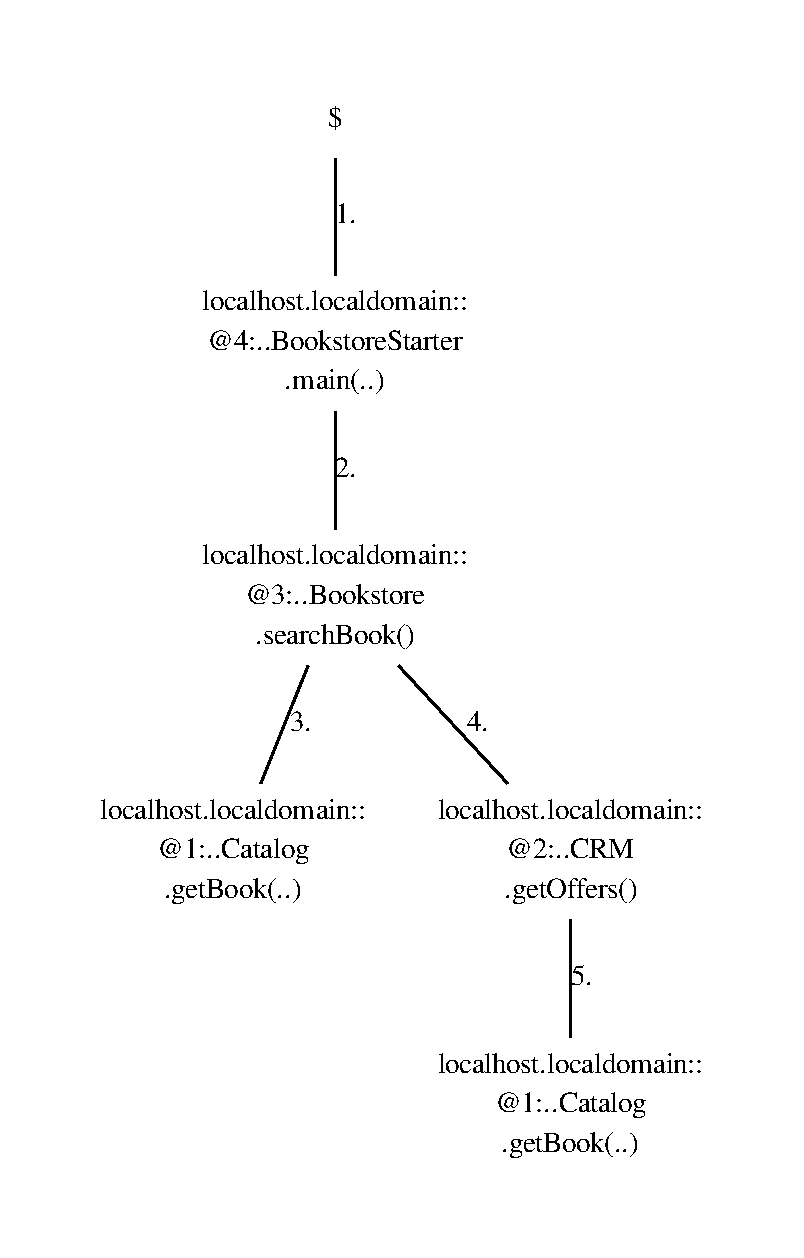
\includegraphics[height=0.4\textheight]{images/callTree}
	}%
	\subfigure[]{\label{fig:traceAnalysis:allocSeqDiagr}%
	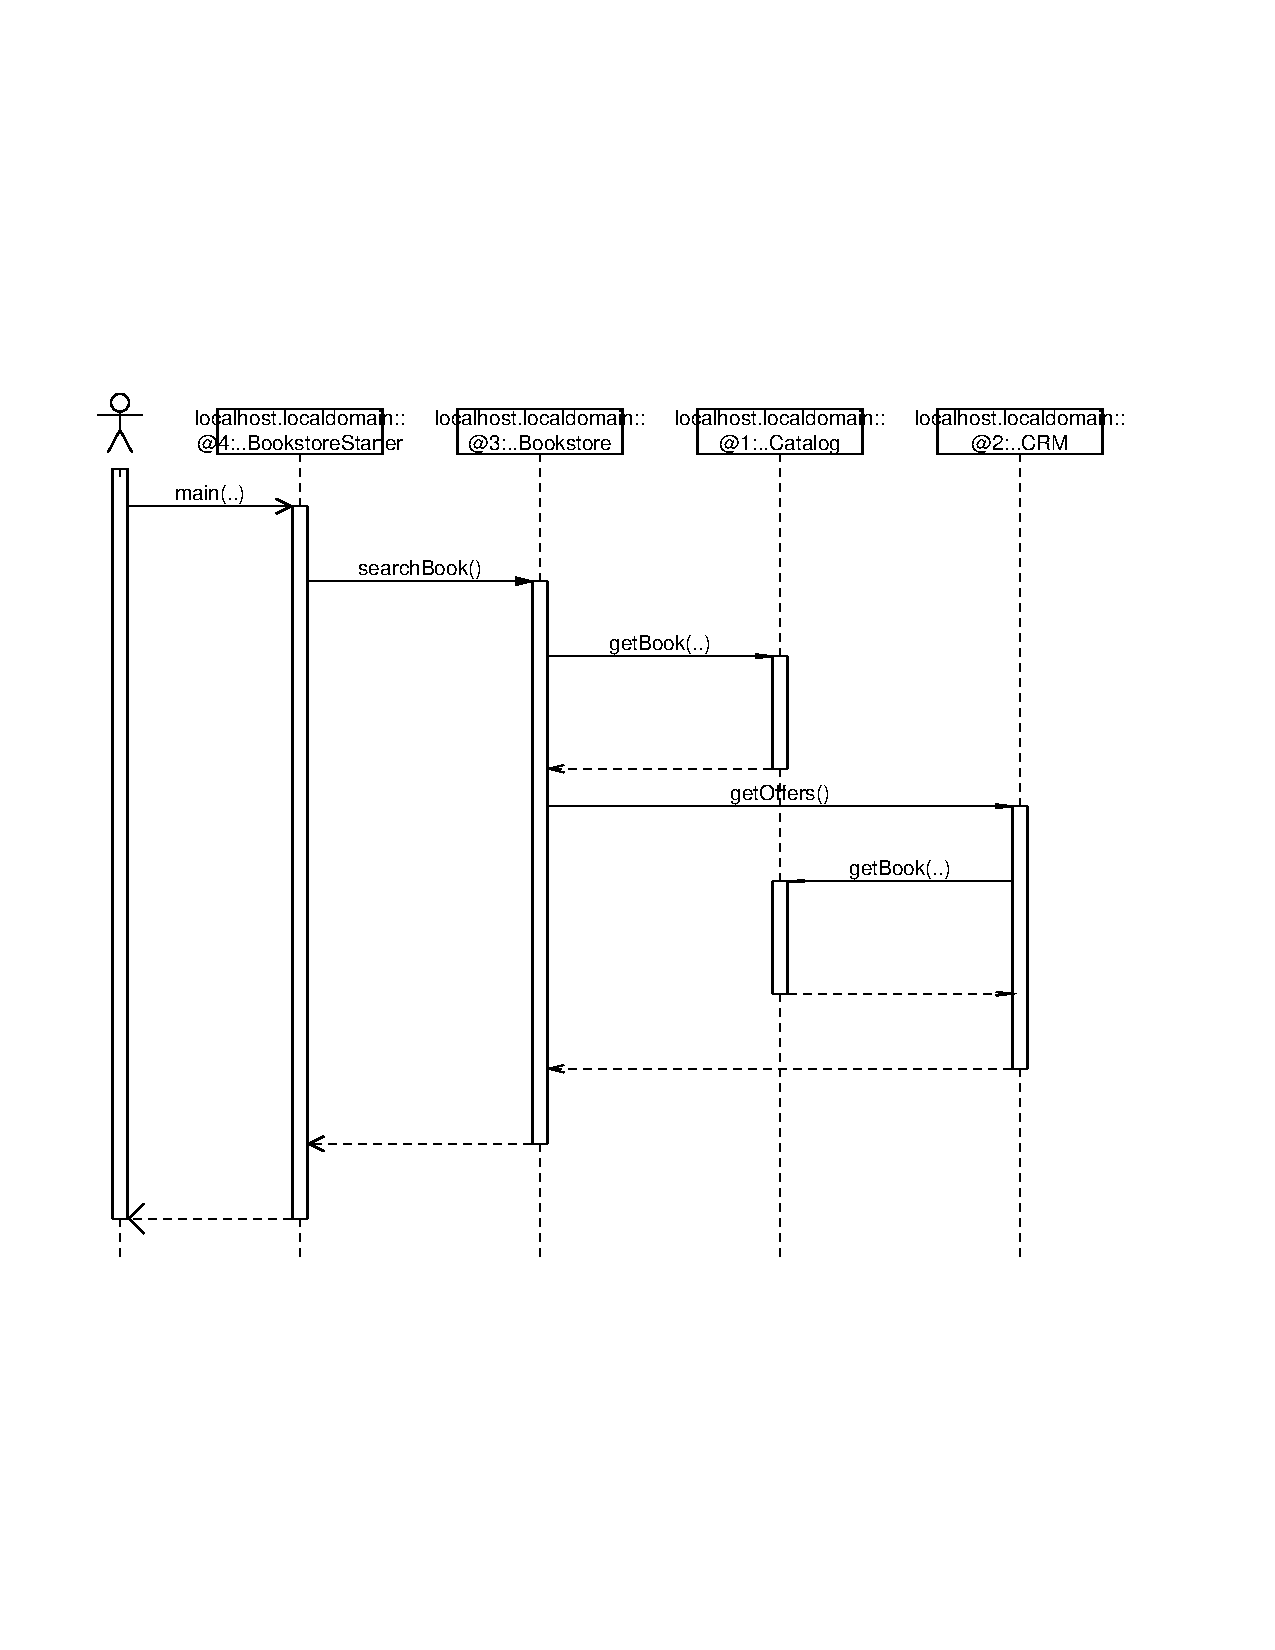
\includegraphics[height=0.4\textheight]{images/allocationSequenceDiagram}
	}%

	\caption{Call Tree~\subref{fig:traceAnalysis:callTree} and Allocation Sequence Diagram~\subref{fig:traceAnalysis:allocSeqDiagr}}
\end{figure}

\NOTIFYBOX{Under Linux it is possible to use a shell script for the converting as well. \file{dotPic-fileConverter.sh} searches all \file{.pic} and \file{.dir}-files in the given directory and converts them by using the necessary tools.}

\section{Full Monitoring}\label{sec:aspectJ:fullweaving}
The full monitoring without using any annotations is quite simple. It is only necessary to modify the corresponding configuration-file of AspectJ, as can be seen in Listing~\ref{lst:aopConfigFileFull}.

\setXMLListing
\lstinputlisting[caption=aop.xml, label=lst:aopConfigFileFull]{ch5-trace-analysis_FullMonitoring-aop.xml}

\noindent The old aspect has been deactivated by removing it (uncommenting it would work as well), while the new aspect \lstinline$<aspect name="kieker.monitoring.probe.aspectJ.executions.OperationExecutionAspectFull"/>$ has been activated. As the name already reveals, the new aspect makes sure that every method within the included classes/packages will be monitored. The exact behavior can be controlled very exactly by using appropriate includes and excludes within the weaver-part of the configuration file. Listing \ref{lst:aopConfigFileFull} shows for example how to make sure that only the methods within the class \class{BookstoreStarter} will be monitored.

The commands to compile and run the source code are just the same as in the Listings~\ref{lst:traceAnalysisCompileRunExample1Win} and \ref{lst:traceAnalysisCompileRunExample1}. The only thing changing is that the annotations within the source code are no longer necessary.

An example log of a complete run can be found in the appendix.

\WARNBOX{By using an own implemented probe it can be necessary to include the corresponding class for this probe as well in the configuration file.}